%\documentclass[wcp,gray]{jmlr} % test grayscale version
\documentclass[wcp]{jmlr}

% The following packages are automatically loaded by jmlr:
% amsmath, amssymb, natbib, graphicx, url, algorithm2e

\usepackage{longtable}
\usepackage{booktabs}

\graphicspath{{figures/}}

% Do not comment the following commands:
\pagenumbering{gobble}
\newcommand{\cs}[1]{\texttt{\char`\\#1}}

\jmlryear{2026}
\jmlrworkshop{ACML 2026}

\title[Static Quantization Is Not a Cross-Platform Reproducibility Primitive]%
{Static Quantization Is Not a Cross-Platform Reproducibility Primitive:\\
A Measurement Study and an Integer-Only Design}

\author{\Name{James Burrell} \Email{jjb2271@columbia.edu}\\
\addr Columbia University}

\editors{Andy Song, Bo Han and Sarah Erfani}

\begin{document}

\maketitle

\begin{abstract}
Floating-point Transformer inference is usually stable enough to deploy, but it
promises no bitwise equality across batch shapes, kernels, or hardware platforms.
It is tempting to treat integer quantization as a fix: an INT8$\times$INT8$\to$INT32
matmul accumulates in exact integer arithmetic, independent of reduction order.
We test this claim with a frozen 286M-parameter NanoChat checkpoint and a
preregistered matrix of seven arithmetic methods across batch sizes 1, 8, and 64,
with 1{,}000 greedy generations per condition, replicated on a second (CPU)
hardware platform. We report three results. First, a \emph{null}: on a single GPU,
batch shape induces no output nondeterminism for any precision: greedy FP32
already matches its own batch-1 reference on 100\% of prompts. Second, a
\emph{nuance}: static W8A8 makes the logits \emph{exactly} batch-invariant (maximum
logit error identical to eight significant figures across batch 1/8/64), and this
holds for both static and dynamic scaling, so the mechanism is integer
accumulation, not scale freezing. Third, and centrally, a \emph{negative result}:
this invariance does not extend across platforms and in fact reverses. Cross-platform
generation agreement (GPU vs.\ CPU) falls from 100\% for FP32 to 85\% (BF16), 45\%
(dynamic W8A8), and 25\% (static W8A8), because normalization, softmax, rotary
embeddings, and dequantization remain floating point and INT8 rounding packs logits
near decision boundaries. We conclude that quantizing only the linear layers cannot
be a cross-platform reproducibility primitive, and we specify the integer-only
design (an op-by-op integerization trained with quantization-aware training) that
would convert batch-invariance into platform-invariance.
\end{abstract}

\begin{keywords}
quantization; reproducibility; determinism; integer-only inference; Transformers
\end{keywords}

\section{Introduction}
Practitioners routinely assume that a fixed model, checkpoint, and prompt yield a
fixed output. In floating point this is false in a subtle way: the IEEE-754
operations used by matrix multiplication are not associative, so the order in which
partial sums are accumulated (which depends on batch shape, the kernel a library
selects, and the hardware it runs on) can change the result in the last few
bits~\citep{pytorch_numerical}. Those bits occasionally propagate through an
$\arg\max$ and change a generated token. Fixing a random seed does not help:
seeding controls sampling, not the numerical path of the forward
pass~\citep{pytorch_reproducibility,he2025nondeterminism}.

Integer quantization is usually motivated by memory and throughput. It also has an
appealing reproducibility property: an integer matmul accumulates in exact
\texttt{int32} arithmetic and is therefore \emph{independent} of accumulation order.
This paper asks whether that property makes static weight-and-activation 8-bit
quantization (W8A8) a \emph{reproducibility primitive}: does a fixed quantization
grid reduce a Transformer's output sensitivity to batch shape and to a change of
hardware platform, relative to FP32/FP16/BF16, and if so, why?

This is a measurement paper with a working prototype, not a completed integer-only
Transformer. Our prototype quantizes only the aligned core linear layers to
INT8$\times$INT8$\to$INT32 and dequantizes for every nonlinear and residual
operation; we use the label \textbf{static W8A8 linear} throughout to keep that
boundary explicit. Our contributions are:
\begin{itemize}
  \item A preregistered measurement of quantization as a reproducibility mechanism,
  with operational definitions separating determinism, reproducibility, and fidelity.
  \item Evidence that integer matmul yields \emph{exact} batch-invariance of logits,
  and that the mechanism is integer accumulation rather than scale freezing.
  \item A cross-platform (GPU vs.\ CPU) result showing that partial (linear-only)
  quantization \emph{degrades} rather than improves reproducibility.
  \item A concrete integer-only design (an op-by-op integerization of a
  non-standard architecture, trained with quantization-aware training) that would
  extend batch-invariance to cross-platform determinism.
\end{itemize}

\section{Motivation and Problem Statement}
\paragraph{Definitions.} We distinguish four properties. \emph{Determinism}: the
same process, run twice, produces identical output. \emph{Repeatability}: identical
output across fresh process launches on the same machine. \emph{Reproducibility}:
identical output across batch shapes, kernels, or platforms. \emph{Fidelity}:
closeness of the output distribution to a chosen FP32 reference. A method can be
perfectly repeatable yet unfaithful, and this distinction drives our results.

\paragraph{Why batch shape and platform matter.} A decode step for a single sequence
and the same step inside a batch of 64 traverse different kernels and reduction
trees; a step on a GPU and on a CPU traverse entirely different implementations.
Because floating-point addition is non-associative and transcendental libraries
differ, the resulting logits can differ. Whether that difference changes a token is
an empirical question, which motivates our design: we hold the model, checkpoint,
prompt, and decoding schedule fixed and vary \emph{only} the physical batch shape,
the arithmetic method, and the hardware platform.

\paragraph{Research question.} Does calibration-fixed W8A8 linear inference reduce
NanoChat's sensitivity to batch shape and to platform relative to floating point,
and is any reduction attributable to fixed scales rather than integer matrix
multiplication alone? We do not equate fixed seeds with deterministic inference, and
we do not claim cross-platform determinism without measuring it.

\section{Related Work}
\paragraph{Integer-only Transformers.} I-BERT~\citep{kim2021ibert} approximates
GELU, softmax, and layer normalization with integer and dyadic arithmetic so that
BERT inference is integer-only; I-ViT~\citep{li2023ivit} extends this to vision
Transformers with integer attention and normalization.
BitNet~\citep{wang2023bitnet} is the most integer-centric training recipe at LLM
scale, learning 1-bit weights from scratch, but its goal is efficiency:
activations, normalization, and attention remain in higher-precision floating
point, so cross-platform bitwise determinism is not among its claims. These works
target accuracy and latency, and they establish that the nonlinear operations we
leave in floating point \emph{can} be made integer, which is precisely the design
we specify in Section~\ref{sec:design}. The integer-arithmetic training of
\citet{jacob2018quantization} underpins modern integer inference.

\paragraph{LLM post-training quantization.} LLM.int8()~\citep{dettmers2022llmint8}
and SmoothQuant~\citep{xiao2023smoothquant} make W8A8 accurate at scale by handling
activation outliers with per-token/per-channel scales and outlier migration;
ZeroQuant~\citep{yao2022zeroquant} adds group-wise scaling with layer-by-layer
distillation, OmniQuant~\citep{shao2024omniquant} learns clipping and equivalent
transformations for weights and activations, and QuaRot~\citep{ashkboos2024quarot}
rotates activations to eliminate outliers, enabling full 4-bit quantization of
weights, activations, and the KV cache. A complementary line compresses
\emph{weights only}: GPTQ~\citep{frantar2023gptq}, AWQ~\citep{lin2024awq},
SpQR~\citep{dettmers2024spqr}, and AQLM~\citep{egiazarian2024aqlm} reach 2--4 bit
weights but keep activations, and hence the matmul accumulation itself, in floating
point; they therefore cannot inherit the order-invariance of integer accumulation,
and we scope them out of this study for that reason. Serving systems such as
Atom~\citep{zhao2024atom} and QServe~\citep{lin2025qserve} do execute low-bit
integer kernels end-to-end, but they select kernels by batch size and hardware to
maximize throughput, which is exactly the variability we measure here. This
literature optimizes accuracy, memory, and throughput; to our knowledge it does not
measure \emph{generation reproducibility} as the primary outcome. Our prototype
uses deliberately minimal per-tensor static activation quantization to isolate the
reproducibility question, which is why its fidelity is below these accuracy-oriented
methods; Section~\ref{sec:design} adopts their per-token scheme.

\paragraph{Cross-platform consistency and framework guidance.} Cross-platform
post-training quantization has been studied where encoder/decoder mismatch is
catastrophic, e.g.\ learned image compression~\citep{yu2022crossplatform}. Vendor
documentation warns that batched and sliced computations need not be bitwise equal
and that determinism requires explicit, performance-costly
flags~\citep{pytorch_numerical,pytorch_reproducibility}. Recent systems work makes
LLM inference batch-invariant by controlling reductions~\citep{he2025nondeterminism};
we instead ask whether quantization achieves invariance as a side effect of integer
accumulation, and find that partial quantization does not achieve it across
platforms.

\section{NanoChat W8A8 Prototype}
\paragraph{Model.} We use a frozen NanoChat~\citep{karpathy2025nanochat} base
checkpoint (\texttt{paper-d12}, step 2520; 12 layers, $d{=}768$, 6 heads, vocabulary
32768; 286{,}261{,}730 parameters; trained on 1.321B tokens; validation BPB 0.8396).
The checkpoint, tokenizer, and prompt/calibration manifests are pinned by SHA-256
and archived with every result directory.

\paragraph{Arithmetic conditions.} FP32 is literal float32 with TF32 disabled; FP16
and BF16 use NanoChat's explicit half-precision paths; deterministic FP32/FP16
controls enable PyTorch deterministic algorithms with a fixed cuBLAS workspace. The
static W8A8 prototype (Algorithm~\ref{alg:w8a8}) uses symmetric INT8 with
per-output-channel weight scales and a per-tensor activation scale frozen from 32
calibration strings; it executes INT8$\times$INT8$\to$INT32 with PyTorch's
\texttt{\_int\_mm} and dequantizes the \texttt{int32} accumulator. The dynamic W8A8
control uses the identical integer matmul but re-estimates the activation scale at
runtime; comparing the two isolates whether any stability comes from the fixed grid
or from integer arithmetic alone.

\begin{algorithm}[t]
\caption{Static W8A8 linear (per-channel weights, per-tensor frozen activation).}
\label{alg:w8a8}
\KwIn{activation $x$; frozen scales $s_a$ (per-tensor), $s_w$ (per-channel);
int8 weights $W_q$; bias $b$}
Calibrate (offline): run the float model on 32 strings; set $s_a = \max|x|/127$\;
$x_q \gets \mathrm{clip}(\mathrm{round}(x / s_a), -127, 127)$ \tcp*{quantize to int8}
\lIf{$\mathrm{rows}(x_q) < 32$}{zero-pad $x_q$ to 32 rows (\texttt{\_int\_mm} constraint)}
$A \gets \texttt{\_int\_mm}(x_q, W_q^\top)$ \tcp*{int8 $\times$ int8 $\to$ int32}
\Return $A_{[:\mathrm{rows}]} \cdot (s_a s_w) + b$ \tcp*{dequantize in fp32}
\end{algorithm}

\paragraph{Claim boundary.} Only aligned core projections are quantized (in/out
features divisible by 8). NanoChat's tiny unaligned smear and value-gate
projections, and all normalization, rotary embedding, attention softmax, residual,
and dequantization operations, remain floating point. This isolates grid snapping
and integer accumulation but is \emph{not} integer-only inference. For decode
matmuls with 16 or fewer rows (which PyTorch's CUDA \texttt{\_int\_mm} rejects), both
W8A8 paths zero-pad to 32 rows and slice the padding from the output.

\section{Experimental Protocol}
The protocol is preregistered and frozen. For every arithmetic
method\,$\times$\,batch size $\in\{1,8,64\}$ we retain exactly 1{,}000 greedy
generations: 20 prompts $\times$ 10 replicas $\times$ 5 fresh process launches. The
final partial logical batch is padded to the declared physical batch size and
padding rows are discarded. The FP32 batch-1 teacher-forced trace is the common
reference. We then replicate the four core methods (FP32, BF16, static/dynamic W8A8)
on a second hardware platform (CPU), where the integer matmul executes but every
surrounding kernel differs from the GPU.

\paragraph{Outcomes.} Generation: unique sequences per prompt across restarts, FP32
batch-1 reference-match rate, modal fraction, and, for cross-platform, whether the
modal token sequence is identical across GPU and CPU. Numerical: mean and maximum
absolute logit difference, logit RMSE, and forward KL from the FP32 batch-1
distribution. Fidelity: held-out validation bits-per-byte (BPB) over 2{,}097{,}152
tokens, throughput, and a static calibration-size sensitivity at 1/8/32 samples.

\paragraph{Statistics.} We report prompt-level means and 95\% prompt-cluster
bootstrap intervals (10{,}000 resamples). Replicas and process launches are repeated
measurements, not independent prompts. Every prespecified condition is reported,
including null results.

\paragraph{Hypotheses.} \textbf{H1} (sanity): FP16 deviates from the FP32 batch-1
reference more than FP32 at batch 8/64. \textbf{H2} (central): static W8A8 has lower
within-condition output multiplicity than FP16 under batch perturbation.
\textbf{H3}: static W8A8 may raise reference-match rate while increasing KL,
separating reproducibility from fidelity. \textbf{H4}: static is more stable than
dynamic W8A8 if scale freezing, rather than integer matmul, is the mechanism.

\section{Results}
\paragraph{A same-machine null result (H1, H2).} On one GPU, batch shape induces
\emph{no} output nondeterminism. Every method at every batch size has unique output
count 1.0 (Table~\ref{tab:main}): each prompt yields a single sequence across all
replicas and launches. FP32 matches its own batch-1 reference on 100\% of prompts at
batch 8/64 despite a nonzero maximum logit drift of $\sim\!1.6\times10^{-5}$; that
drift never crosses an $\arg\max$ boundary. H1 holds directionally, but H2 finds no
multiplicity to reduce: FP16 and BF16 are already output-deterministic across batch
on this machine.

\begin{table}[t]
\centering
\caption{Greedy matrix (1{,}000 generations per row). $|\Delta|$ is absolute logit
difference from the FP32 batch-1 reference; KL is forward KL in nats; BPB is held-out
validation fidelity. Static/dynamic W8A8 use calibration 32.}
\label{tab:main}
\footnotesize
\begin{tabular}{llrrrrr}
\toprule
Method & Batch & Match & Mean$|\Delta|$ & Max$|\Delta|$ & KL & BPB \\
\midrule
FP32 & 1 & 1.00 & 0.00e+00 & 0.00e+00 & 2.18e-09 & 0.8395 \\
FP32 & 8 & 1.00 & 1.08e-06 & 1.32e-05 & 2.29e-09 & 0.8395 \\
FP32 & 64 & 1.00 & 1.74e-06 & 1.62e-05 & 5.23e-09 & 0.8395 \\
\addlinespace
FP16 & 1 & 0.95 & 3.22e-03 & 2.34e-02 & 2.31e-06 & 0.8395 \\
FP16 & 8 & 0.95 & 3.21e-03 & 2.33e-02 & 2.33e-06 & 0.8395 \\
FP16 & 64 & 0.95 & 3.19e-03 & 2.42e-02 & 2.33e-06 & 0.8395 \\
\addlinespace
BF16 & 1 & 0.75 & 2.56e-02 & 1.83e-01 & 1.46e-04 & 0.8396 \\
BF16 & 8 & 0.70 & 2.56e-02 & 1.80e-01 & 1.46e-04 & 0.8396 \\
BF16 & 64 & 0.70 & 2.57e-02 & 1.85e-01 & 1.47e-04 & 0.8396 \\
\addlinespace
Static W8A8 & 1 & 0.00 & 6.92e-01 & 4.88e+00 & 9.55e-02 & 0.8752 \\
Static W8A8 & 8 & 0.00 & 6.92e-01 & 4.88e+00 & 9.55e-02 & 0.8752 \\
Static W8A8 & 64 & 0.00 & 6.92e-01 & 4.88e+00 & 9.55e-02 & 0.8752 \\
\addlinespace
Dynamic W8A8 & 1 & 0.15 & 3.52e-01 & 3.48e+00 & 3.42e-02 & 0.8761 \\
Dynamic W8A8 & 8 & 0.15 & 3.52e-01 & 3.48e+00 & 3.40e-02 & 0.8761 \\
Dynamic W8A8 & 64 & 0.15 & 3.52e-01 & 3.48e+00 & 3.40e-02 & 0.8761 \\
\addlinespace
\bottomrule
\end{tabular}

\end{table}

\paragraph{Exact batch-invariance from integer matmul (H4).} Where floats carry
small batch-dependent noise, the integer paths do not. Static W8A8's maximum logit
error is identical to eight significant figures across batch 1/8/64
(Table~\ref{tab:main}, Figure~\ref{fig:logit}), so its logits are exactly invariant
to batch shape, which FP32 is not. Dynamic W8A8 is likewise invariant. Because both
the fixed-scale and runtime-scale variants are exactly invariant, \textbf{H4 is not
supported}: the reproducibility mechanism is exact integer accumulation, not scale
freezing.

\begin{figure}[t]
\centering
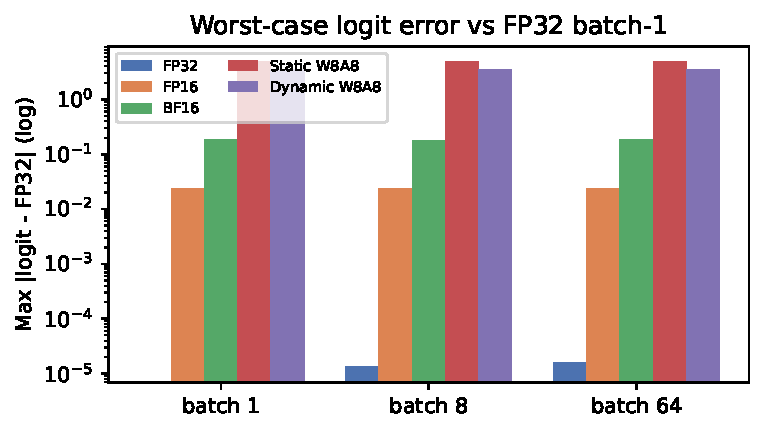
\includegraphics[width=0.7\textwidth]{fig3_logit_error.pdf}
\caption{Worst-case logit error vs.\ FP32 batch-1 (log scale). FP32 batch-1 is zero
by construction; float error grows slightly with batch, while W8A8 error is large
but \emph{constant} across batch shape.}
\label{fig:logit}
\end{figure}

\paragraph{Reproducibility is not fidelity (H3).} The invariance is purchased by
computing a different function. Static W8A8 matches the FP32 reference on 0\% of
prompts and dynamic on 15\%; static W8A8's mean KL from FP32 is 0.095 nats versus
$2.3\times10^{-6}$ for FP16. Validation BPB rises from 0.8395 (FP32) to 0.8752
(static) and 0.8761 (dynamic), whereas FP16/BF16 stay within $10^{-4}$ of FP32
(Table~\ref{tab:fidelity}). H3 is confirmed: a W8A8 model can be perfectly
repeatable and batch-invariant while being a worse approximation of FP32.

\begin{table}[t]
\centering
\caption{Fidelity ablation: held-out validation BPB over 2.1M tokens.}
\label{tab:fidelity}
\footnotesize
\begin{tabular}{llr}
\toprule
Method & Calib.\ samples & Validation BPB \\
\midrule
BF16 & -- & 0.83959 \\
Dynamic W8A8 & -- & 0.87612 \\
FP16 & -- & 0.83954 \\
FP32 & -- & 0.83954 \\
Static W8A8 & 1 & 0.87715 \\
Static W8A8 & 8 & 0.87509 \\
Static W8A8 & 32 & 0.87520 \\
\bottomrule
\end{tabular}

\end{table}

\paragraph{Where precision flips tokens.} Reproducibility risk is content-dependent
(Table~\ref{tab:categories}). Under FP16/BF16, factual, numerical, reasoning, and
instruction prompts match the FP32 reference on 100\% of cases, while
\emph{completion} and \emph{ambiguous} prompts flip most often (BF16 33\% each).
These are prompts whose top logits are nearly tied, so a $10^{-2}$-scale
perturbation crosses the decision boundary. With two or three prompts per category this is
a descriptive signal, but it indicates that any reproducibility budget should be
spent on open-ended generation rather than factual recall.

\begin{table}[t]
\centering
\caption{Per-category reference-match rate (batch 1). Lower means the precision
flips more tokens relative to FP32.}
\label{tab:categories}
\footnotesize
\begin{tabular}{lrrrr}
\toprule
Category & FP16 & BF16 & Static W8A8 & Dynamic W8A8 \\
\midrule
Factual & 1.00 & 1.00 & 0.00 & 0.00 \\
Reasoning & 1.00 & 1.00 & 0.00 & 0.33 \\
Numerical & 1.00 & 1.00 & 0.00 & 0.50 \\
Technical & 1.00 & 0.67 & 0.00 & 0.00 \\
Instruction & 1.00 & 1.00 & 0.00 & 0.00 \\
Completion & 0.67 & 0.33 & 0.00 & 0.00 \\
Ambiguous & 1.00 & 0.33 & 0.00 & 0.33 \\
\bottomrule
\end{tabular}

\end{table}

\paragraph{The central negative result: cross-platform (CPU).} We replicate the core
methods on a CPU platform and measure whether the modal generated token sequence per
prompt is identical on GPU and CPU (Table~\ref{tab:crossplatform},
Figure~\ref{fig:crossplatform}). The outcome is the opposite of the naive
expectation. FP32 reproduces the same text on \textbf{100\%} of prompts across
platforms: at full precision the GPU$\leftrightarrow$CPU logit gap never crosses an
$\arg\max$ boundary. Agreement then \emph{falls} as precision drops: BF16 85\%,
dynamic W8A8 45\%, static W8A8 only \textbf{25\%}. Partial quantization is thus
markedly \emph{worse} for cross-platform reproducibility than full precision. The
mechanism compounds two effects: integer accumulation removes batch-dependent
variation, but INT8 rounding packs many logits near decision boundaries, and the
surrounding floating-point operations (dequantization, normalization, softmax,
rotary) use different kernels on CPU than on GPU. No method here produces
bit-identical logits across platforms; FP32 merely has enough headroom that its
argmax is unchanged.

\begin{table}[t]
\centering
\caption{Cross-platform replication: fraction of prompts whose modal greedy token
sequence is identical on GPU and CPU (batch 1).}
\label{tab:crossplatform}
\footnotesize
\begin{tabular}{lr}
\toprule
Method & GPU$\leftrightarrow$CPU text match \\
\midrule
FP32 & 100.0\% \\
BF16 & 85.0\% \\
Static W8A8 & 25.0\% \\
Dynamic W8A8 & 45.0\% \\
\bottomrule
\end{tabular}

\end{table}

\begin{figure}[t]
\centering
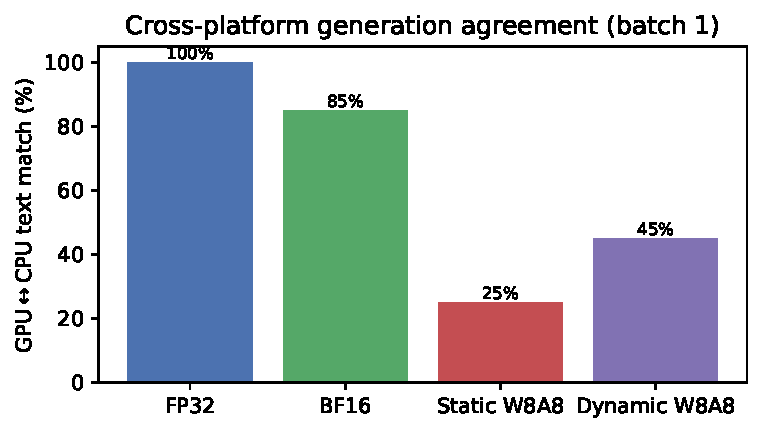
\includegraphics[width=0.7\textwidth]{fig5_crossplatform.pdf}
\caption{GPU$\leftrightarrow$CPU generation agreement. Full precision is already
platform-stable at the token level; lower precision diverges, and linear-only
quantization is the worst. The remaining floating-point operations prevent bitwise
platform invariance.}
\label{fig:crossplatform}
\end{figure}

\section{Design: An Integer-Only Path to Platform Invariance}
\label{sec:design}
The negative result has a clear cause: only the linear layers are integer, so the
argmax-determining path still runs through platform-divergent floating-point
operations. We specify the design that would remove them. It is a design and
feasibility analysis; we have not yet trained or evaluated it.

\paragraph{Determinism, not compression, sets the bit-widths.} Because the goal is
identical bits rather than smaller tensors, only the large matmuls need to be INT8;
the nonlinear operations can use wide INT32 fixed-point, which preserves accuracy
while remaining exactly reproducible. Table~\ref{tab:intspec} maps each NanoChat
operation to its integer replacement. Two operations are effectively free: relu$^2$
is exact in integer, and the monotone \texttt{tanh} softcap does not change a greedy
argmax and can be dropped.

\begin{table}[t]
\centering
\caption{Op-by-op integerization of NanoChat. Widths are chosen for determinism.}
\label{tab:intspec}
\footnotesize
\begin{tabular}{lll}
\toprule
Operation & Float today & Integer target \\
\midrule
Core linears & fp matmul & INT8$\times$INT8$\to$INT32 + dyadic requant \\
RMSNorm (no-param) & \texttt{rms\_norm} & integer inverse-sqrt (Newton), int32 \\
Attention QK$^\top$/$\times$V & fp (flash-attn) & integer matmul + requant \\
Softmax & fp exp/$\div$ & I-BERT integer exp + integer normalize \\
Rotary $x_1c{+}x_2s$ & fp tables & fixed-point cos/sin (Q15) \\
relu$^2$ & fp & integer square (exact) \\
sigmoid gates & fp & integer LUT \\
resid/x0/backout $\lambda$ & fp mul & dyadic fixed-point scalar \\
Embeddings & fp table & per-channel int8 table \\
softcap $15\tanh(z/15)$ & fp & dropped (monotone $\Rightarrow$ argmax-preserving) \\
Logits & fp & int32 (argmax directly) \\
\bottomrule
\end{tabular}
\end{table}

\paragraph{Quantization-aware training with train/inference parity.} Post-training
integerization of a checkpoint not trained for it risks incoherent output on a weak
286M model: ``deterministic garbage.'' The accurate route is quantization-aware
training (QAT): simulate integer rounding in the forward pass with a straight-through
estimator while keeping fp32 master weights for the optimizer, using per-token
activation scales (which, unlike our per-tensor prototype, control outliers). The
non-negotiable correctness requirement is \emph{parity}: the fake-quant forward used
in training must be arithmetically identical to the integer inference path, so the
trained model is exactly the deployed model. A warm-started QAT finetune from
\texttt{paper-d12} for a fraction of the original tokens is the low-cost first step.

\paragraph{Expected outcome and the determinism metric.} If the entire path is
integer, the int32 logits are computed with no non-associative float reductions and
no platform-specific transcendental libraries, so the SHA-256 hash of the logit
tensor should be identical across batch 1/8/64 and across GPU/CPU, while every method
in Table~\ref{tab:crossplatform} differs. This converts the batch-invariance we
already observe (Table~\ref{tab:main}) into the platform-invariance we do not.

\section{Discussion, Threats, and Roadmap}
\paragraph{A null result is informative.} For this model on this GPU, greedy
same-machine inference is already batch-invariant at the token level; quantization is
not needed to stabilize same-machine batching, and using it for that purpose forfeits
fidelity for no reproducibility gain. The defensible positive claim is narrower and
exact: integer matmul yields bitwise-identical logits across batch shapes, which
matters for applications that compare log-probabilities rather than only tokens.

\paragraph{Threats to validity.} (i) One model, one checkpoint, and two platforms
cannot establish generality. (ii) FP32's same-machine and cross-platform stability is
regime-dependent (small model, greedy decoding, short 32-token generations, high
precision); it would not survive sampling, long sequences, or near-tie-heavy prompts,
as the category analysis suggests. (iii) Our prototype uses minimal per-tensor
activation quantization, so its cross-platform result partly reflects quantization
quality; however, the floating-point islands are a barrier that better quantization
cannot remove, which is why Section~\ref{sec:design} integerizes them. (iv) The
padding compatibility path and the remaining float operations are confounds for any
strict determinism claim.

\paragraph{Roadmap.} Build the integer-only path of Section~\ref{sec:design}, verify
train/inference parity, train a QAT checkpoint to fidelity within $\sim$0.02 BPB of
FP32, and re-run this matrix plus a 1{,}000-completion end-to-end test, reporting
logit-hash agreement across batch and platform.

\section{Conclusion}
Studied as a reproducibility primitive, static W8A8 delivers exactly what integer
accumulation promises (logits invariant to batch shape) but no more: it is a
different, lower-fidelity function, and its invariance not only fails to survive a
change of hardware platform but reverses, dropping cross-platform text agreement from
100\% (FP32) to 25\%, because most of the network is still floating point and INT8
logits sit near decision boundaries. Batch-invariance and platform-invariance are
distinct goals, and only the former follows from integer matmul alone. A genuinely
integer-only inference path, trained with quantization-aware training, is the route
from one to the other, and is the natural next step.

\bibliography{references}

\end{document}
